% Online supplement. Compiles standalone; no citations, so no bibliography.
\documentclass[11pt]{article}
\usepackage[margin=2.8cm]{geometry}
\usepackage{amsmath,amssymb}
\usepackage{graphicx}
\graphicspath{{figs_v2/}}
\usepackage{booktabs}
\usepackage{multirow}
\usepackage[hidelinks]{hyperref}

\renewcommand{\thesection}{S\arabic{section}}
\renewcommand{\thetable}{S\arabic{table}}
\renewcommand{\thefigure}{S\arabic{figure}}

\title{Online supplement to:\\
\emph{Completion-aware search with partial witness repair for dense
fixed-shape facility layout}}
\author{Junhwan Ahn \and Kunwoo Lee \and Kyunghyun Lee \and Yeoneung Kim}
\date{}

\begin{document}
\maketitle

\noindent This supplement contains four secondary experiments
referenced from the main text: zero shot transfer (\ref{app:transfer}),
quality and diversity fronts (\ref{app:qd}), amortized cost (\ref{app:amortize})
and action granularity (\ref{app:granularity}), followed by the full
improvement formulation ablation (\ref{app:ablation}), a qualitative
certificate gallery (\ref{app:gallery}), the complete MCNC/GSRC conversion
(\ref{app:conversion}) and the large instance feasibility record
(\ref{app:bigbench}). Each experiment follows the protocol in the main text.
The main claims do not depend on these experiments, and we report the relevant
control for each experiment. Section S9 gives the full budget sensitivity and
mechanism record for the comparison in which all methods start from the same
layout.
Section S10 collects the diagnostic evidence removed from the shortened main
text; complete run-level outputs remain in the archive.

\section{Zero shot transfer}
\label{app:transfer}
A trained policy can have an advantage through amortization. A solver restarts
for every brief, while a policy evaluates a new brief in one forward pass. We
trained a policy only on procedurally generated briefs. The type inventory,
dimensions, affinity tables, plate aspect ratio, fill ratio, wall preferences
and objective constants were randomized during $1.2$M training steps. We then
evaluated the policy on briefs that were not optimized during training.

\begin{table}[htbp]
\centering
\caption{Zero shot transfer at $n=32$. The greedy constructor provides the
direct comparison because, like the policy, it does not search over the plate.
It also requires no training. Its cost is $32$ and $528$ marginal objective
sweeps per layout; the batched figure on the heterogeneous generated set is
higher, so we report the cost for one instance.}
\label{tab:transfer}
\footnotesize
\setlength{\tabcolsep}{4pt}
\begin{tabular}{@{}lrrrrr@{}}
\toprule
 & & & \multicolumn{2}{c}{greedy constructive} & RL zero shot \\
\cmidrule(lr){4-5}
test set & shelf & SA 45k lat. & area ord. & room+pos. & ($\times16$+pol.) \\
\midrule
generated (in distribution) & 1\,912.6 & \textbf{2\,613.9} & 2\,488.8 & 2\,597.5 & 2\,591.0 \\
\textsc{office} (unseen) & 2\,942.5 & 3\,412.1 & 3\,359.5 & 3\,380.2 & \textbf{3\,426.3} \\
\textsc{clinic} (unseen) & 3\,503.7 & 4\,011.9 & 3\,955.6 & \textbf{4\,116.5} & 3\,950.2 \\
\midrule
evaluations/layout & 1 & 58\,963 to 65\,875 & 32 & 528 & 2\,049 to 5\,633 \\
\bottomrule
\end{tabular}
\end{table}

\begin{figure}[htbp]
\centering

\includegraphics[width=\linewidth]{fig_transfer.pdf}
\caption{Held out briefs, annotated with objective evaluations per layout. The
two reference scenarios were authored by hand and never optimized in training.
The RL bars show $16$ samples without the final polish ($512$ evaluations), a
cheaper operating point than the $\times16$+polish column of
Table~\ref{tab:transfer}, which is why the two differ slightly.}
\label{fig:transferapp}
\end{figure}

On \textsc{office} the zero shot policy reaches $3\,414.5$ with a single greedy
decode ($32$ evaluations, $12.7$\,ms), matching annealing's $3\,412.1$ at
$60\,371$ evaluations, and $3\,426.3$ with $16$ samples and a polish. At the same
$32$ evaluations the constructor without training reaches $3\,359.5$.

\textsc{clinic} gives a different result. The greedy constructor reaches
$4\,116.5$, which is higher than both full budget annealing and the zero shot
policy. At a matched $32$ evaluations,
it reaches $3\,955.6$ against the policy's $3\,848.5$. Across the three test sets
the zero shot policy is better on one, similar on one and worse on one. These
results show that one set of weights can evaluate unseen briefs with a quality
similar to large budget annealing while using three to four orders of magnitude
less search. They do not show that the policy is always better. Transfer is
evaluated at a fixed facility count
(main text, Limitations).

\section{Quality and diversity}
\label{app:qd}
A common argument for learning in design is that a policy provides a
\emph{distribution} over layouts. Previous comparisons used one policy
temperature and several annealing budgets. We vary all three methods. We vary
the sampling temperature for the policy, the budget for annealing, and the
fraction of randomized commitments for the constructor without training.

\begin{table}[htbp]
\centering
\caption{Quality against diversity on \textsc{office}, $64$ samples from one
start. Diversity is the mean pairwise fraction of cells whose room type differs,
estimated from $400$ of the $2\,016$ pairs, so it carries about $\pm0.01$ of
sampling noise; every row uses the same estimator.}
\label{tab:qd}
\footnotesize
\begin{tabular}{@{}lrrr@{}}
\toprule
method & $J$ & diversity & ms/sample \\
\midrule
policy, order chosen by policy, $T{=}1.0$   & 3\,529.3 & 0.006 & 22 \\
policy, random commit order, $T{=}1.0$      & 3\,508.0 & 0.304 & 19 \\
\quad $T{=}2.5$                             & 3\,418.2 & 0.405 & 18 \\
\quad $T{=}5.0$                             & 3\,048.0 & 0.623 & 13 \\
\midrule
SA 8\,192, lattice                          & 3\,321.1 & 0.581 & 478 \\
SA 45\,000, lattice                         & 3\,414.5 & 0.639 & 1\,070 \\
\midrule
greedy constructive, area order             & 3\,359.5 & 0.000 & 7 \\
\quad $20\%$ of commit slots reshuffled     & 3\,374.5 & 0.350 & 114 \\
\quad $50\%$                                & 3\,408.3 & 0.482 & 251 \\
\quad $70\%$                                & \textbf{3\,415.2} & 0.531 & 294 \\
\quad $100\%$                               & 3\,405.2 & 0.620 & 347 \\
\bottomrule
\end{tabular}
\end{table}

\begin{figure}[htbp]
\centering

\includegraphics[width=\linewidth]{fig_qd.pdf}
\caption{Quality against diversity with all three sides swept. Faint markers are
points that a method's own front dominates.}
\label{fig:qdapp}
\end{figure}

We make three observations. First, a policy whose entropy bonus is annealed to
zero produces almost no diversity. At $T{=}1$, its diversity is $0.006$. Second,
randomizing the commit order increases diversity by a factor of fifty with a
$0.6\%$ decrease in objective. Third, applying the same procedure to the greedy
rule produces its own front. Randomizing a controlled fraction of the commit
slots changes diversity continuously from $0.000$ to $0.620$ and reaches $3\,415.2$ at
diversity $0.531$ for $32$ objective evaluations, which matches the best
annealing point anywhere on the front ($3\,414.5$ at $0.639$, $61\,267$
evaluations).

The two fronts cross once. The policy has a higher objective up to diversity
$\approx0.42$, while the constructor without training has a higher objective above
$\approx0.45$. An earlier, coarser
sweep of the heuristic, which tried only a uniform random order and therefore
jumps from $0.000$ to $0.603$, suggested a gap in its range that does not
exist. This is a single scenario result and we did not repeat it on the suite.

\section{Amortized cost}
\label{app:amortize}
Training has a fixed initial cost, while search has a cost for every layout.
Table~\ref{tab:amortize} reports the annealing budget sweep on
\textsc{office}, each budget's
wall clock time per layout, and the first point on the policy's training curve
($488$ recorded checkpoints, $2\,049$\,s total) at which the policy's greedy
decode exceeds that budget's mean objective. The policy finishes at $3\,529.3$
and decodes in $17.8$\,ms per layout.

\begin{table}[htbp]
\centering
\caption{Annealing budget against the training time needed to match it. The
$45$k lattice row is the measurement of the main comparison (the budget
sweep's own $45$k run gives $3\,400.8$ at $1.13$\,s); the larger budgets come
from the dedicated sweep. The legacy scenario implementation is not batched, so its
time per layout is omitted.}
\label{tab:amortize}
\footnotesize
\begin{tabular}{@{}lrrr@{}}
\toprule
annealer & mean $J$ & s/layout & training s to exceed \\
\midrule
legacy scenario implementation, $45$k & 3\,269.9 & not reported & 109 \\
lattice, $45$k   & 3\,414.8 & 1.00 & 157 \\
lattice, $150$k  & 3\,459.0 & 3.40 & 215 \\
lattice, $400$k  & 3\,489.1 & 8.83 & 256 \\
lattice, $10^{6}$ & 3\,501.3 & 20.08 & 268 \\
\bottomrule
\end{tabular}
\end{table}

Charging the full $2\,049$\,s up front and $17.8$\,ms per layout thereafter,
the policy has a lower total wall clock cost than annealing with $10^{6}$
evaluations after $2049/(20.08-0.018)\approx102$ layouts. Compared with lattice
annealing using $45\,000$ evaluations, this occurs after
$2049/(1.00-0.018)\approx2\,093$ layouts.

This comparison has two limitations. First, the workload contains repeated
requests for the \emph{same} brief. An annealer could store its best layout and
reuse it for later requests. A stream of unseen briefs is evaluated separately
in \ref{app:transfer}. Second, this comparison is against annealing and not
against the constructor without training. At $88$\,ms per layout, the initial
training cost is recovered only after roughly $29\,000$ layouts relative to the
constructor. Thus, amortization does not provide an advantage over this
constructor for smaller workloads.

\section{Action granularity}
\label{app:granularity}
We compare a discrete action head for small moves with a continuous displacement
head when feasibility is handled by a penalty. Our earlier experiments on a
small scenario suggested a tradeoff between feasibility and return, but they
were conducted before the present protocol and are not used as evidence. We
report the comparison inside
the corrected improvement MDP on the single $n=32$ \textsc{office} scenario
(best observed reward, jump and swap moves, Metropolis acceptance). One checkpoint
per action head is evaluated from the same 64 independent random starts, shown in
Table~\ref{tab:granularity}. No tradeoff appears in this evaluation. With
sampled decoding at horizon $4\,096$ the lattice head reaches $3\,069.6$ at
$50\%$ feasibility while the continuous head reaches $2\,737.0$ at $0\%$, and
deterministic decoding of either head falls into a limit cycle and loses more
than a thousand objective units. The feasible-volume record in
Table~\ref{tab:sfeasvol} explains the direction geometrically, and under the constructive
formulation the question does not arise.

\begin{table}[htbp]
\centering
\caption{Discrete against continuous action head inside the corrected
improvement MDP on \textsc{office}, $n=32$: mean and standard deviation across
the same 64 independent evaluation starts.}
\label{tab:granularity}
\footnotesize
\begin{tabular}{@{}llrrr@{}}
\toprule
head & decode & horizon & $J$ & feasible \\
\midrule
discrete (lattice) & sampled & 512    & $2\,475.3\pm93.8$  & 0.00 \\
discrete (lattice) & sampled & 2\,048 & $2\,853.0\pm101.4$ & 0.06 \\
discrete (lattice) & sampled & 4\,096 & $3\,069.6\pm126.3$ & 0.50 \\
discrete (lattice) & argmax  & 4\,096 & $1\,372.6\pm228.4$ & 0.00 \\
continuous & sampled & 512    & $2\,354.7\pm76.2$  & 0.00 \\
continuous & sampled & 2\,048 & $2\,611.4\pm85.5$  & 0.00 \\
continuous & sampled & 4\,096 & $2\,737.0\pm60.8$  & 0.00 \\
continuous & mean    & 4\,096 & $1\,649.5\pm203.9$ & 0.00 \\
\bottomrule
\end{tabular}
\end{table}

\section{Improvement formulation ablation, in full}
\label{app:ablation}
The main text summarizes the corrections to the improvement MDP on
\textsc{office}; Table~\ref{tab:ablationfull} gives every variant. Each is
trained for a matched budget of $688$k environment steps and evaluated on $64$
held out starts using stochastic decoding at $4\,096$ objective evaluations.

\begin{table}[htbp]
\centering
\caption{Improvement formulation ablation on \textsc{office}.}
\label{tab:ablationfull}
\footnotesize
\begin{tabular}{@{}llrr@{}}
\toprule
ID & configuration & $J$ & feasible \\
\midrule
A0 & reference: difference reward, translate, $\gamma{=}0.995$ & 2\,658.5 & 0\,\% \\
A0$'$ & the same with $\gamma{=}0$                              & 1\,804.3 & 0\,\% \\
A1 & \quad + best observed reward                                 & 2\,246.1 & 0\,\% \\
A2 & \quad + best observed reward, jump and swap                  & 2\,461.8 & 0\,\% \\
C1 & \quad + Metropolis accept/reject (lattice head)            & \textbf{3\,067.2} & \textbf{48\,\%} \\
C1$'$ & the same with a continuous head                         & 2\,737.0 & 0\,\% \\
\midrule
\multicolumn{2}{@{}l}{A0 evaluated deterministically (argmax)}   & 1\,445.5 & 0\,\% \\
\bottomrule
\end{tabular}
\end{table}

\section{Certificate gallery}
\label{app:gallery}
Figure~\ref{fig:gallery} shows one held out instance at fill ratio $0.95$
solved by the same largest first constructor under the four certificate
settings of the main text's certificate comparison. Without a certificate the
constructor occupies too much free space in the early steps, and the last
facilities have no legal position;
the scalar objective reports this only as a lower number.

\begin{figure}[htbp]
\centering
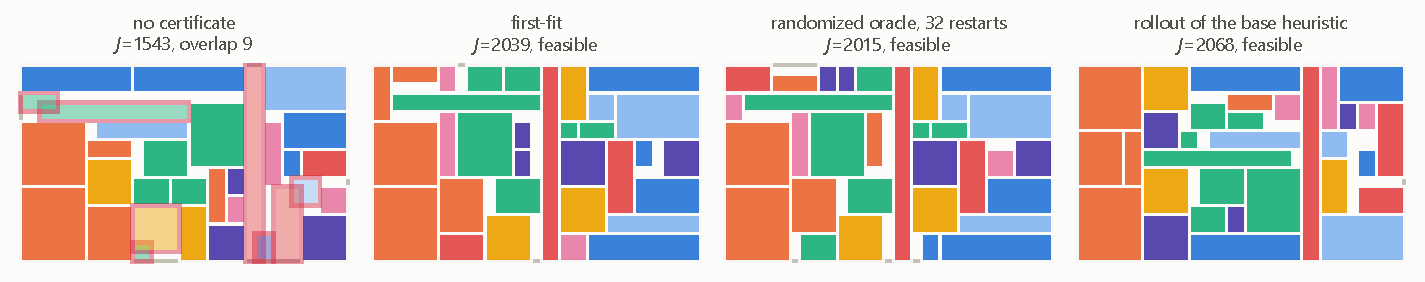
\includegraphics[width=\linewidth]{fig_gallery.pdf}
\caption{One instance, four certificates, same constructor. Facilities that
end up overlapping are outlined in red.}
\label{fig:gallery}
\end{figure}

\section{MCNC/GSRC conversion, in full}
\label{app:conversion}
HPWL numbers depend on the conversion, so we state it completely. Block
dimensions come from the GSRC \texttt{.blocks} files
(\texttt{hardrectilinear} records, width and height from the corner list);
netlists from the UCLA \texttt{.nets} files; terminal positions from the
\texttt{.pl} files, matched to net pins by name. Pins are placed at block centers and
terminals at their given coordinates, the standard simplification. Nets with
fewer than two pins are dropped, contributing zero. Coordinates are divided by
an integer for each instance and floored, which is necessary because the legality
masks are dense over the plate: the factor is $6$ for \textsc{ami33}, $33$
for \textsc{ami49} and $3$ for the GSRC instances, chosen as the smallest
divisor bringing the plate under $200$ cells per side, and it is reported with
every result. The outline is fixed by area,
$\text{plate}=\text{total block area}/(1-\text{dead space})$, at aspect
ratio $1$; blocks may be rotated by $90^\circ$. Under this conversion HPWL is
comparable across the paper's own methods but not against published
floorplanning numbers, which use full resolution and a different pin model.
Integer flooring changes block shapes and packing possibilities, so converted
dead space is not treated as a published full-resolution result.

\section{Larger instances}
\label{app:bigbench}
Table~\ref{tab:bigbench} gives the full feasibility record of the
constructors without training on $96$ to $256$ facilities summarized in the main
text.

\begin{table}[htbp]
\centering
\caption{Constructors without training on larger instances, feasibility rate.
Every instance has a verified feasible packing, so a failure indicates that the
method did not find the existing packing.
Plate geometry is drawn per cell, so rows are not comparable with one another;
the comparison is between methods within a row. The rollout certificate is
$O(n^2WH)$ per query and was not run above $128$ facilities; that is recorded
rather than omitted.}
\label{tab:bigbench}
\footnotesize
\begin{tabular}{@{}lrccc@{}}
\toprule
$n$ & instances & no certificate & first fit & rollout \\
\midrule
\multicolumn{5}{@{}l}{\emph{fill ratio 0.85}} \\
\quad 96  & 15 & 1.00 & 1.00 & 1.00 \\
\quad 128 & 15 & 1.00 & 1.00 & 1.00 \\
\quad 192 & 15 & 1.00 & 1.00 & not run \\
\quad 256 & 15 & 1.00 & 1.00 & not run \\
\midrule
\multicolumn{5}{@{}l}{\emph{fill ratio 0.95}} \\
\quad 96  & 30 & 0.57 & 0.53 & \textbf{0.90} \\
\quad 128 & 30 & 0.53 & 0.57 & \textbf{0.90} \\
\quad 192 & 30 & 0.70 & 0.63 & not run \\
\quad 256 & 30 & 0.83 & 0.83 & not run \\
\bottomrule
\end{tabular}
\end{table}

\section{Complete results for methods starting from the same layout}
\label{app:sharedfull}

Every row below uses a common verified best-contact layout and retains it as a
feasible incumbent. Stochastic seeds are averaged within an instance before
cell means are computed. The 0.1 and 0.3 second values are read from the same
anytime run that continues to 1.0 second. Times exclude the common measured
initialization cost, which is charged equally to all methods in total-time
reporting. Mean initialization and verification time ranges from 0.0052 to
0.0128 seconds over the four cells. All normalized improvements use the full
feasible objective $J_\beta$, including the constant no-overlap bonus.

\begin{table}[htbp]
\centering
\caption{Dense confirmation at fill 0.95. Entries are mean percentage
improvement over the common initial layout.}
\label{tab:sharedfull}
\small
\setlength{\tabcolsep}{4pt}
\begin{tabular}{@{}llrrrrrrrr@{}}
\toprule
geometry & $n$ & sec. & B1 & B2 & B2S & B3 & M0 & R0 & M1 \\
\midrule
guillotine & 32 & 0.1 & 1.72 & 0.55 & 0.82 & 2.45 & 3.50 & 1.64 & \textbf{6.14} \\
            &    & 0.3 & 1.72 & 1.22 & 1.82 & 4.37 & 7.59 & 1.96 & \textbf{7.83} \\
            &    & 1.0 & 1.72 & 2.40 & 3.51 & \textbf{9.63} & 9.04 & 2.43 & 9.51 \\
guillotine & 64 & 0.1 & 0.00 & 0.22 & 0.41 & 1.29 & \textbf{1.72} & 0.21 & 1.41 \\
            &    & 0.3 & 4.20 & 0.68 & 0.87 & 2.21 & 3.64 & 1.33 & \textbf{5.21} \\
            &    & 1.0 & 4.44 & 1.41 & 1.62 & 3.69 & 8.00 & 2.31 & \textbf{8.76} \\
nonslicing & 32 & 0.1 & 1.79 & 0.57 & 1.02 & 1.95 & 3.50 & 1.91 & \textbf{6.32} \\
            &    & 0.3 & 1.79 & 1.43 & 2.03 & 4.13 & 7.63 & 2.27 & \textbf{7.83} \\
            &    & 1.0 & 1.79 & 2.64 & 3.71 & 9.53 & \textbf{10.15} & 2.86 & 9.65 \\
nonslicing & 64 & 0.1 & 0.00 & 0.18 & 0.44 & \textbf{1.64} & 1.47 & 0.13 & 1.14 \\
            &    & 0.3 & 3.46 & 0.74 & 0.96 & 2.31 & 2.56 & 1.46 & \textbf{4.68} \\
            &    & 1.0 & 4.10 & 1.38 & 1.78 & 3.60 & 7.78 & 2.70 & \textbf{7.98} \\
\bottomrule
\end{tabular}
\end{table}

\begin{table}[htbp]
\centering
\caption{Pooled M1 minus control contrasts on 196 initialized dense instances.
Entries are percentage points with paired instance-bootstrap 95\% intervals.}
\label{tab:sharedcontrasts}
\scriptsize
\setlength{\tabcolsep}{2.4pt}
\begin{tabular}{@{}rrrrrrr@{}}
\toprule
sec. & B1 & B2 & B2S & B3 & M0 & R0 \\
\midrule
0.1 & 2.84 [2.26,3.45] & 3.32 [2.83,3.82] & 3.03 [2.56,3.52] & 1.87 [1.36,2.39] & 1.18 [0.58,1.75] & 2.75 [2.33,3.17] \\
0.3 & 3.55 [2.57,4.49] & 5.35 [4.84,5.86] & 4.95 [4.47,5.43] & 3.12 [2.58,3.67] & 1.05 [0.46,1.67] & 4.61 [4.12,5.10] \\
1.0 & 5.93 [4.99,6.88] & 7.02 [6.54,7.52] & 6.33 [5.84,6.82] & 2.41 [1.74,3.06] & 0.25 [$-0.42$,0.92] & 6.39 [5.89,6.92] \\
\bottomrule
\end{tabular}
\end{table}

At 1.0 second, the raw M1 minus B1 difference is 224.5 objective units
[172.2,276.5], its win/tie/loss count is 156/0/40, and 152 of 196 instances
exceed the one-percent practical threshold. The corresponding counts against
B2, B2S, M0 and R0 are 196/0/0, 195/0/1, 109/0/87 and 195/0/1. The M0 interval
does not establish a difference.

\begin{table}[htbp]
\centering
\caption{Boundary study at fill 0.90 and 1.0 second. Entries are mean
percentage improvement over the common initial layout. The last column is the
paired M1 minus B1 percentage-point difference with a 95\% bootstrap interval.}
\label{tab:sharedboundary}
\footnotesize
\setlength{\tabcolsep}{3.5pt}
\begin{tabular}{@{}llrrrrrrrrr@{}}
\toprule
geometry & $n$ & init. & B1 & B2 & B2S & B3 & M0 & R0 & M1 & M1$-$B1 \\
\midrule
guillotine & 32 & 20/20 & 13.03 & 7.89 & 7.60 & 8.84 & \textbf{16.17} & 7.97 & 14.60 & 1.57 [$-0.27$,3.65] \\
guillotine & 64 & 20/20 & 14.06 & 5.53 & 4.94 & 4.70 & \textbf{15.48} & 6.25 & 13.44 & $-0.62$ [$-2.09$,1.07] \\
nonslicing & 32 & 19/20 & 11.86 & 6.92 & 7.28 & 9.43 & \textbf{14.90} & 8.03 & 13.84 & 1.97 [$-0.07$,4.02] \\
nonslicing & 64 & 20/20 & 14.98 & 5.01 & 4.82 & 4.10 & \textbf{15.85} & 6.68 & 13.07 & $-1.91$ [$-3.54$,$-0.25$] \\
\bottomrule
\end{tabular}
\end{table}

\begin{table}[htbp]
\centering
\caption{Mechanism log at fill 0.95 and 1.0 second. Repair success is
conditional on a nonempty displaced set with size at most four. Verified
completions exclude the carried fallback. R0 contains reuse only, and M0 uses
full regeneration for every nonfallback proposal.}
\label{tab:repairmechanism}
\small
\begin{tabular}{@{}llrrrrrr@{}}
\toprule
geometry & $n$ & mean $|D|$ & repair success & M1 reuse & M1 verified & R0 verified & M0 verified \\
\midrule
guillotine & 32 & 1.95 & 2.45\% & 14.0 & 80.8 & 26.4 & 59.6 \\
guillotine & 64 & 2.49 & 3.91\% & 6.4 & 61.1 & 23.8 & 40.9 \\
nonslicing & 32 & 2.05 & 2.19\% & 15.9 & 76.1 & 29.7 & 59.0 \\
nonslicing & 64 & 2.72 & 3.55\% & 6.9 & 55.0 & 26.2 & 35.7 \\
\bottomrule
\end{tabular}
\end{table}

Across all dense M1 runs, the repair branch produces 6,215 incumbent updates
and 142,270 objective units of logged gain; unchanged reuse produces 1,380
updates and 12,455 units. These event counts are mechanism descriptions rather
than inferential samples. B2 and B2S have mean destroy sizes 8.88 to 9.06 and
2.99, respectively.

\begin{table}[htbp]
\centering
\caption{Mean measured work per one-second dense run, in milliseconds. Late is
the number of candidates that completed after the cutoff and were discarded.}
\label{tab:sharedtiming}
\small
\begin{tabular}{@{}lrrrrrr@{}}
\toprule
method & generation & intermediate verify & final verify & objective & return time & late \\
\midrule
B1  & 0.0 & 0.0 & 0.1 & 0.1 & 1001.53 & 0 \\
B2  & 0.0 & 0.0 & 2.9 & 2.6 & 1002.58 & 1 \\
B2S & 0.0 & 0.0 & 15.6 & 13.5 & 1002.67 & 14 \\
B3  & 845.4 & 37.7 & 40.3 & 40.9 & 1001.44 & 28 \\
M0  & 719.3 & 21.4 & 30.7 & 30.6 & 1001.26 & 23 \\
R0  & 0.0 & 12.6 & 105.0 & 92.9 & 1001.66 & 81 \\
M1  & 358.1 & 30.3 & 65.2 & 61.8 & 1001.11 & 47 \\
\bottomrule
\end{tabular}
\end{table}

All 8,820 dense budget layouts and 5,214 boundary budget layouts pass an
independent result audit. Recomputed objective and trace selection errors are
zero. No admitted dense event is later than 0.999998 seconds. Nonpreemptive
work can return up to 9.8 ms after the cutoff, but its candidate is not admitted.
The adversarial regression set rejects duplicate and missing
facilities, negative and out-of-range coordinates, overlap, stale witnesses and
incomplete timeout returns, while accepting legal edge contact.

\section{Diagnostic evidence omitted from the focused main text}
\label{app:legacydiagnostics}

These experiments motivated completion-aware construction but are not evidence
for the primary matched-time claim. Table~\ref{tab:sfeasvol} shows why an overlap
penalty receives little feasible exploration as size and density increase. The
lattice column is higher than the continuous-center column wherever both are
resolved, so action representation matters before learning.

\begin{table}[htbp]
\centering
\caption{Fraction of uniformly sampled layouts that are overlap free. Each
entry averages four generated instances at $4\times10^4$ samples; $<6\times
10^{-6}$ means no feasible sample was drawn.}
\label{tab:sfeasvol}
\scriptsize
\setlength{\tabcolsep}{3pt}
\begin{tabular}{@{}lrrrrrr@{}}
\toprule
 & \multicolumn{2}{c}{fill 0.35} & \multicolumn{2}{c}{fill 0.50}
 & \multicolumn{2}{c}{fill 0.65} \\
\cmidrule(lr){2-3}\cmidrule(lr){4-5}\cmidrule(lr){6-7}
$n$ & continuous & lattice & continuous & lattice & continuous & lattice \\
\midrule
2  & $2.6\times10^{-1}$ & $3.7\times10^{-1}$ & $1.7\times10^{-1}$ & $2.4\times10^{-1}$ & $7.1\times10^{-2}$ & $1.4\times10^{-1}$ \\
4  & $3.3\times10^{-2}$ & $7.6\times10^{-2}$ & $3.0\times10^{-3}$ & $1.5\times10^{-2}$ & $5.0\times10^{-4}$ & $3.9\times10^{-3}$ \\
6  & $4.0\times10^{-3}$ & $1.7\times10^{-2}$ & $1.6\times10^{-4}$ & $1.1\times10^{-3}$ & $<6\times10^{-6}$ & $2.5\times10^{-5}$ \\
8  & $5.9\times10^{-4}$ & $4.5\times10^{-3}$ & $1.9\times10^{-5}$ & $6.9\times10^{-5}$ & $<6\times10^{-6}$ & $<6\times10^{-6}$ \\
10 & $8.8\times10^{-5}$ & $1.1\times10^{-3}$ & $<6\times10^{-6}$ & $1.3\times10^{-5}$ & $<6\times10^{-6}$ & $<6\times10^{-6}$ \\
12 & $6.3\times10^{-6}$ & $2.2\times10^{-4}$ & $<6\times10^{-6}$ & $<6\times10^{-6}$ & $<6\times10^{-6}$ & $<6\times10^{-6}$ \\
16 & $<6\times10^{-6}$ & $1.3\times10^{-5}$ & $<6\times10^{-6}$ & $<6\times10^{-6}$ & $<6\times10^{-6}$ & $<6\times10^{-6}$ \\
\bottomrule
\end{tabular}
\end{table}

The earlier single-facility improvement MDP used the reward
$J(s_{t+1})-J(s_t)$. With discount one it optimizes the terminal objective; with
discount below one it favors high intermediate values and penalizes recovered
detours. At a common 688k-step training budget, adding a best-observed reward,
jump and swap moves, and Metropolis acceptance raised the objective from
$2\,658.5$ to $3\,067.2$ and feasibility from 0\% to 48\%. Lattice annealing
reached $3\,414.8$, and a masked constructor without training reached
$3\,380.2$. Table~\ref{tab:ablationfull} gives the complete formulation ablation.

Initialization was also a major confound in the old decoder. On 100-instance
dense cells $(n,f)=(32,0.90),(32,0.95),(64,0.95)$, bottom-left fill in area
order covered 0.78, 0.09 and 0.28; best-contact covered 0.98, 0.96 and 1.00.
This is why every primary method now receives the same archived best-contact
layout. The legacy exact-marginal selector matched or exceeded the two learned
selectors in most $n=64$ cells, so learning is not used in M1.

Finally, the learned completion predictor was trained on 25,258 rollout states
with an instance-grouped split. Validation AUC was 0.902, but on disjoint fill
0.95 tests its best completion rate was 0.20, compared with 0.90 for verified
first fit and 1.00 for the more expensive rollout certificate. The labels record
success of one heuristic rollout, not true membership in the set of completable
states. This negative result supports learned candidate ordering, but not using
an unverified classifier as a hard feasibility decision.

\end{document}
